\chapter{Software Implementation and Experimental Verification}

After the basic hardware behavior of Phaser was established, the next step was to test its practical use through a series of simple but representative programming tasks. The goal of this stage was not only to verify that the board could produce the expected outputs, but also to develop a software interface that could expose the useful parts of Phaser in a form suitable for repeated experimental use. The implementation was written as an ARTIQ experiment so that waveform parameters could be adjusted from the dashboard while the actual output updates remained inside kernel code and therefore stayed under deterministic timing control \cite{artiq_rtio, artiq_coredrivers, artiq_phaser_module}.

\subsection{Single-frequency output test}

The first test was a single-frequency output. This was used as the most basic verification that one oscillator could be programmed correctly and that the resulting output appeared as a single spectral component rather than a distorted or multi-component waveform. In practical terms, this test checked the most fundamental control path: board initialization, channel selection, attenuation setting, carrier placement, oscillator programming, and DUC update.

Figure~\ref{fig:single_tone_test} shows the result of this measurement. A single isolated peak is observed, which indicates that the programmed tone was generated successfully and that the basic signal chain was functioning as intended. This test served as the starting point for the more structured tests that followed.

\begin{figure}[t]
    \centering
    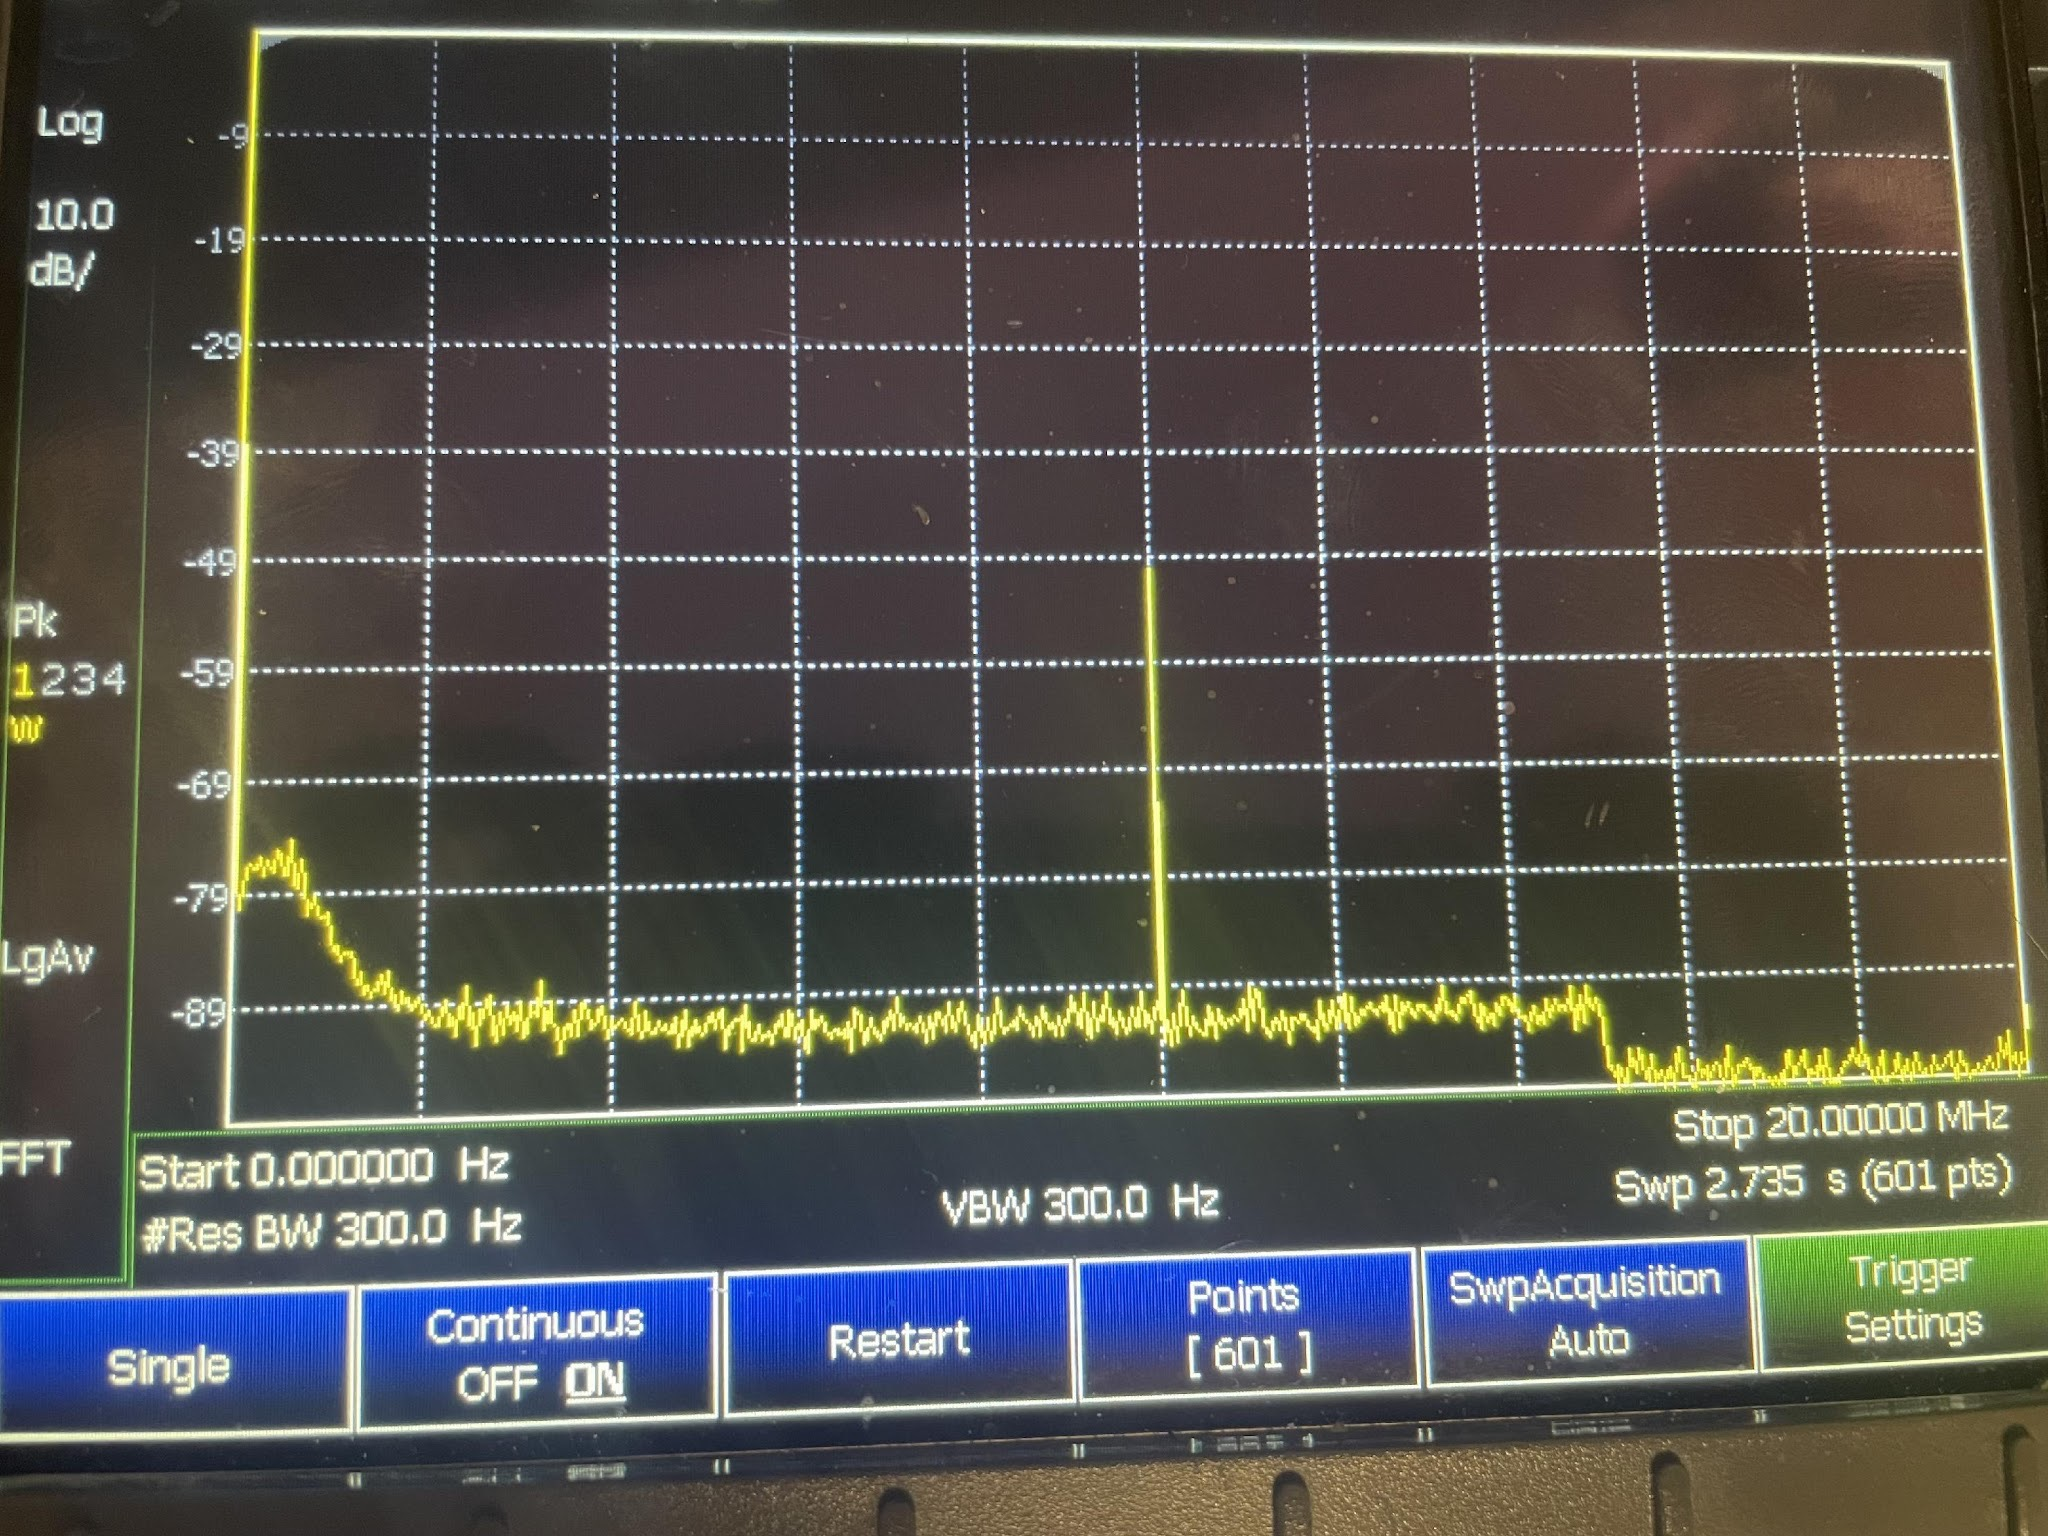
\includegraphics[width=0.62\linewidth]{Pictures/single.jpg}
    \caption{Single-frequency output test. The appearance of one dominant spectral line was used as the first verification of correct oscillator and channel programming.}
    \label{fig:single_tone_test}
\end{figure}

\subsection{Single-channel multitone output}

After the single-tone case was verified, the next step was to test whether one Phaser channel could produce more than one frequency at the same time. This is one of the main practical differences between Phaser and a simpler single-tone RF source. In the Phaser software model, one channel contains five oscillators, so several tones can be defined independently and then summed into one channel output \cite{artiq_phaser_module, artiq_coredrivers}.

The multitone test was performed by programming two different oscillator frequencies on the same channel. The result is shown in Fig.~\ref{fig:double_tone_test}. Two clearly resolved spectral peaks are visible. This confirms that the channel can carry more than one programmed frequency simultaneously and that the oscillator summation works in the expected way. For quantum experiments, this capability is important because it allows one RF path to carry a structured signal rather than only one carrier. This is useful for bichromatic driving, sideband-based control, or other pulse schemes in which more than one spectral component must remain phase-related within the same output channel.

\begin{figure}[t]
    \centering
    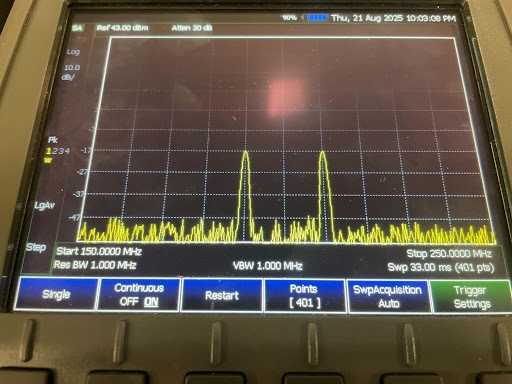
\includegraphics[width=0.62\linewidth]{Pictures/double_frequency.jpg}
    \caption{Single-channel multitone output. Two distinct spectral peaks are observed from one Phaser channel, confirming successful simultaneous generation of two programmed frequencies.}
    \label{fig:double_tone_test}
\end{figure}

\subsection{Two-channel relative phase test}

Frequency control alone is not sufficient for many quantum-control tasks. Relative phase between channels is also important, especially when two RF paths are intended to interfere, to remain synchronized, or to define a repeatable optical phase relation. For this reason, a separate test was carried out for relative phase control.

In this test, one channel was used as the reference output. The second channel was programmed at the same frequency, but with additional phase offsets of 0.25, 0.5, and 0.75 turns. These values correspond to quarter-cycle, half-cycle, and three-quarter-cycle offsets. The resulting traces are shown in Fig.~\ref{fig:phase_test}. The output waveforms show the expected relative shifts, which verifies that the programmed phase offsets are reflected in the output signal in a consistent way.

This result is important because it shows that Phaser can be used not only for frequency synthesis but also for controlled inter-channel phase relationships. In practice, this is one of the signal properties that most directly affects the quality of coherent experimental control. The ARTIQ documentation also notes that absolute-phase-sensitive updates should be aligned to frame boundaries when deterministic latency is required, which is consistent with the way this type of test should be scheduled in real experiments \cite{artiq_coredrivers, artiq_phaser_module}.

\begin{figure}[t]
    \centering
    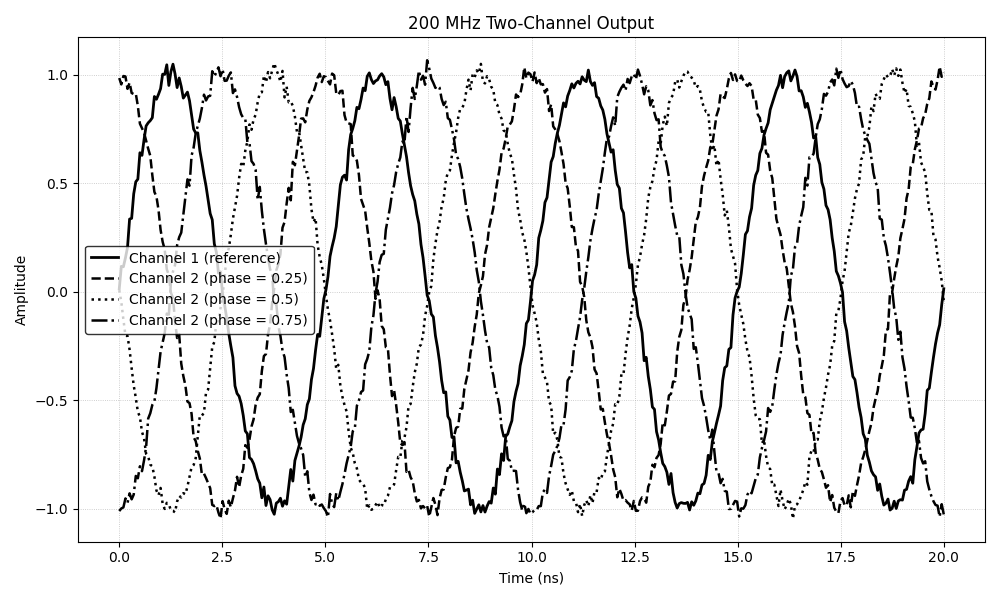
\includegraphics[width=0.82\linewidth]{Pictures/phase.png}
    \caption{Relative phase test between two channels. Channel 1 is used as a reference, while Channel 2 is programmed with relative phase offsets of 0.25, 0.5, and 0.75 turns.}
    \label{fig:phase_test}
\end{figure}

\subsection{Amplitude-sequenced output}

In addition to frequency and phase control, amplitude scheduling was also tested in order to verify that burst-style output patterns could be programmed in a controlled way. Figure~\ref{fig:amplitude_test} shows a waveform with several gated intervals, where the output amplitude is increased step by step and separated by off periods. This type of sequence is relevant for experiments that need pulsed RF application, staged power ramps, or basic envelope control during calibration and debugging.

Although this test is simpler than a fully shaped pulse, it is still useful because it demonstrates that the software can coordinate repeated on/off timing with controlled changes in oscillator amplitude. This is also consistent with the sequential-output mode implemented later in the main interface.

\begin{figure}[t]
    \centering
    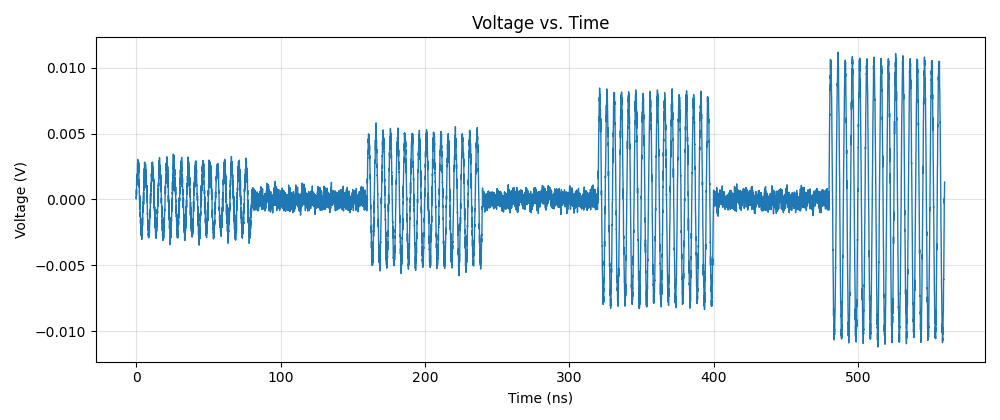
\includegraphics[width=0.78\linewidth]{Pictures/amplitude.png}
    \caption{Amplitude-sequenced output used to verify gated bursts with increasing output level and intervening off periods.}
    \label{fig:amplitude_test}
\end{figure}

\subsection{Full user interface for two-channel Phaser control}

After the individual tests above were completed, a more complete user interface was written so that the useful parts of Phaser could be accessed directly from the ARTIQ dashboard. The final experiment was implemented as the class \texttt{phaserShowcase}, and it was designed to use both Phaser channels while exposing the main control parameters in a simple experimental interface.

At the highest level, the interface supports three operating modes: sequential output, parallel output, and a combined mode that performs both. It also exposes global timing controls such as the gap between sequential bursts and the duration of the parallel burst. For each channel, the user can set attenuation and carrier frequency. In addition, each of the five oscillators on each channel has its own frequency, amplitude, phase, and sequential duration setting. This gives full per-tone control while still keeping the interface manageable from the dashboard.

The structure of this interface matches the practical logic of Phaser operation. Channel-level settings are used for attenuation and carrier placement, while oscillator-level settings are used for the individual tones. Before output is programmed, the code checks that the sum of oscillator amplitudes on a channel does not exceed unity. This is an important safeguard, since Phaser forms the channel output by summing the oscillator contributions. In sequential mode, one tone is programmed, held for its assigned duration, and then turned off before the next tone is applied. In parallel mode, all programmed tones are loaded together and emitted simultaneously for the selected burst time. The relevant DUC update is then strobed so that the staged settings take effect in the output path \cite{artiq_coredrivers, artiq_phaser_module}.

Figure~\ref{fig:interface_test} shows the resulting dashboard interface. The practical value of this interface is that it exposes most of the useful functionality of one Phaser board without requiring the user to rewrite the kernel logic for each new test. It therefore serves both as a debugging tool and as a reusable control layer for future experiments involving multitone generation, phase control, and timed RF sequences.

\begin{figure}[t]
    \centering
    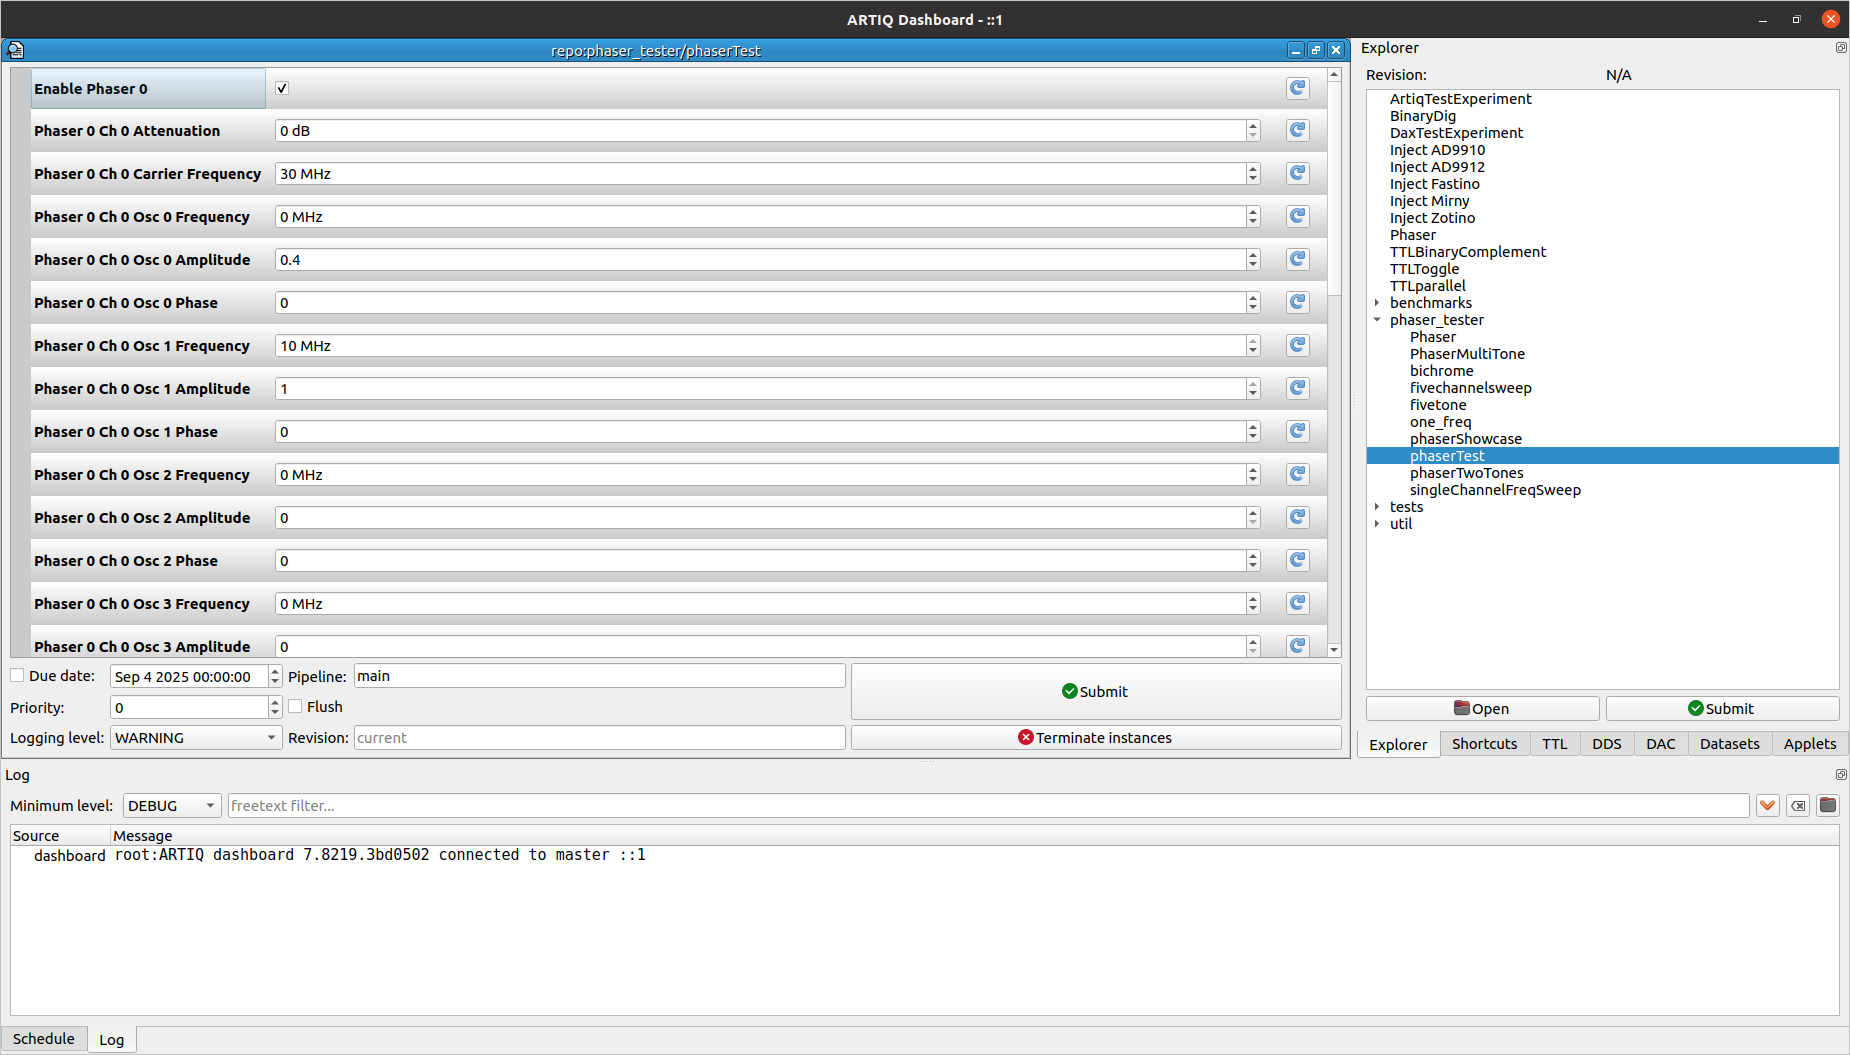
\includegraphics[width=0.95\linewidth]{Pictures/interface.png}
    \caption{Dashboard interface for the final Phaser control program. The interface exposes per-channel attenuation and carrier settings, as well as per-oscillator frequency, amplitude, and phase controls for both channels.}
    \label{fig:interface_test}
\end{figure}

